\subsection{Examples} \label{chapter4:execution-models:examples}

\subsubsection{Illustration Of The Fluxional Exection Model}

\marginfig{9}{0.4\textwidth}{
  
\includegraphics[height=0.2\textwidth]{../resources/grumpy.png}
}

Even if the fluxional execution model is not designed to directly develop applications, a first application was develop directly with it, to test it.
This application doesn't use the transformation, nor the continuous development advocated in this thesis.
Nonetheless, it is related here to illustrate the basic functioning of the fluxional execution model.

The application is accessible online at \url{http://grumpy.etnbrd.com}, and the source code is available at \url{https://github.com/etnbrd/grumpy}.
And the network of fluxions structuring the applications can be monitored in realtime at \url{http://grumpy.etnbrd.com/console}, as illustrated in figure \ref{fig:grumpy-screenshot}.
The application allows to post anonymous grumbles into chat rooms.
Additionally, a room can subscribe to the grumbles from another room.
The reader is invited to play with this application and the monitoring console to maybe quickly grasp an understanding of the fluxional execution model \footnote{The reader might want to keep in mind that crude languages might be present on the platform. It is available freely on the internet for anyone to express itself.}.

\begin{figure}
  \bigfig{
    \centering
    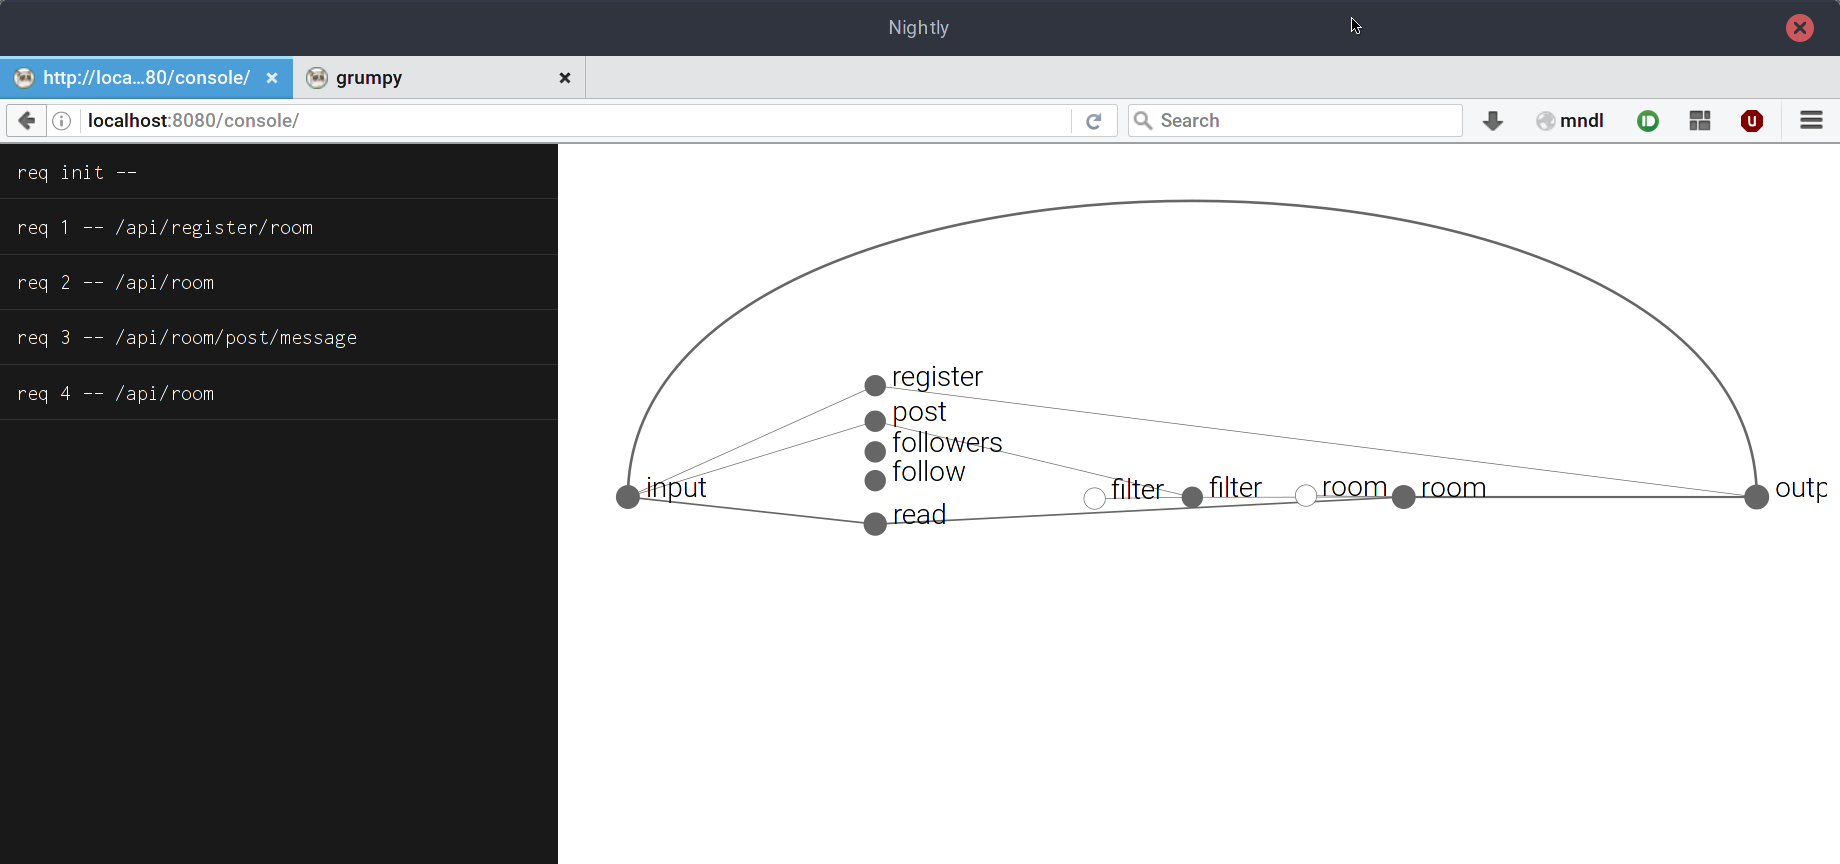
\includegraphics[width=\textwidth]{../resources/grumpy-console.png}
    \caption{Screenshot from the grumpy console}
    \label{fig:grumpy-screenshot}
  }
\end{figure}

The network of fluxions is organized into five layers of stages, traversed by the stream of request from left to right.
The first and last layers are the input and output, connecting the application with the clients.
The second layer contains the fluxions receiving and formatting the request, before passing them to the next layer.
The fluxion in the third layer is a simple filter before posting grumbles.
It is an example of a fluxion modifying a message from the stream.
Finally, each room is instantiated as a new fluxion in the fourth layer, storing the received grumbles in its context.

The left panel logs the requests received by the application, and the path of each request can be traced from stage to stage.

The socket descriptor is stuck with the network interface, hence, it cannot be serialized to flow from one fluxion to another.
Instead, the first and last fluxions share their memory, and each request flows with an id to associate it with its socket descriptor.

This example application was developed before the implementation of the isolation of fluxions in the fluxional execution model.
So it was possible to share their memory by simply sending a memory reference between two fluxions, without grouping them.
This explains the direct link between the input and output fluxions.

The example illustrated in the next paragraphs explains in more details the transformation, and the grouping required for fluxion sharing memory.
And it explains the impact of the memory dependencies on parallelism and scalability.

\subsubsection{Illustration Of The Application Transformation}

The transformation from continuation passing style to the fluxion execution model is now illustrated with a simple web application.

\begin{code}[js,
  caption={Example web application},
  label={lst:source}]
var app = require('express')(),
    fs = require('fs'),
    count = 0; //@\label{lst:source-counter}@

app.get('/', function handler(req, res){ //@\label{lst:source-handler}@
  fs.readFile(__filename, function reply(err, data) {
    count += 1;
    res.send(err || template(count, data)); //@\label{lst:source-send}@
  });
}); //@\label{lst:source-handler-end}@

app.listen(8080);
\end{code}

% \begin{wrapfigure}{r}{0.60\textwidth}
%   \vspace{-25pt}
%   \begin{center}
%     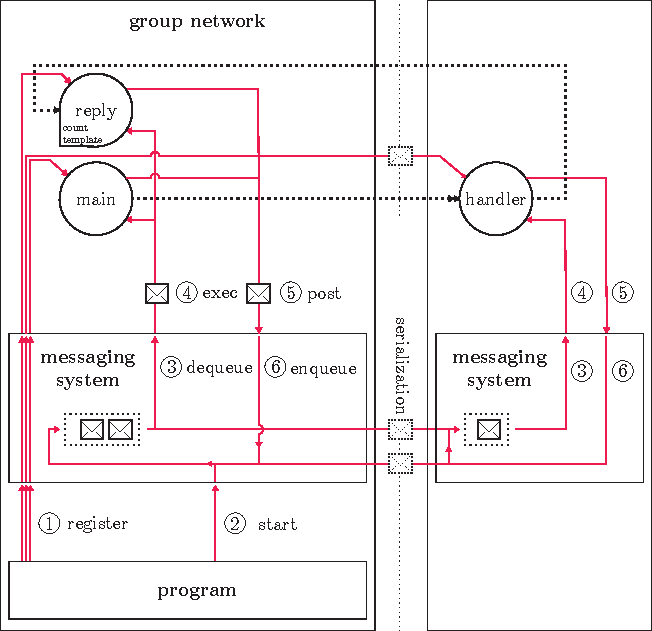
\includegraphics[width=\linewidth]{../resources/schema-message.pdf}
%     \caption{The fluxional execution model in details}
%     \label{fig:MesSys}
%   \end{center}
%   \vspace{-10pt}
% \end{wrapfigure}

% The fluxional execution model is illustrated with an example application presented in listing \ref{lst:source}.
The example application in listing \ref{lst:source} reads a file, and sends it back along with a request counter.
The \texttt{handler} function, line \ref{lst:source-handler} to \ref{lst:source-handler-end}, receives the input stream of requests.
The \texttt{count} variable at line \ref{lst:source-counter} counts the requests, and needs to be saved between two messages receptions.
The \texttt{template} function formats the output stream to be sent back to the client.
The \texttt{app.get} and \texttt{res.send} functions, lines \ref{lst:source-handler} and \ref{lst:source-send}, interface the application with the clients.
Between these two interface functions, there is a chain of three functions to process the client requests : \texttt{app.get} $\to$ \hspace{-1.4em} $\to$ \texttt{handler} $\to$ \texttt{reply}.
This chain of functions is transformed into a pipeline, expressed in the high-level fluxional language in listing \ref{lst:fluxional}.
The transformation process between the source and the fluxional code is explained in chapter \ref{chapter5}, in section \ref{chapter5:flx:compiler}.

\begin{code}[flx, caption={Example application expressed in the high-level fluxional language}, label={lst:fluxional}]
flx main & grp_res
>> handler [res]
  var app = require('express')(),
      fs = require('fs'),
      count = 0;

  app.get('/', >> handler); //@\label{lst:fluxional-streamtohandler}@
  app.listen(8080);

flx handler
-> reply [res]
  function handler(req, res) {
    fs.readFile(__filename, -> reply); //@\label{lst:fluxional-readfile}@
  }

flx reply & grp_res {count, template}
-> null
  function reply(error, data) {
    count += 1; //@\label{lst:fluxional-counter}@
    res.send(err || template(count, data)); //@\label{lst:fluxional-ressend}@
  }
\end{code}

The execution is illustrated in figure \ref{fig:MesSys}.
The dashed arrows between fluxions represent the message streams as seen in the fluxional application.
The plain arrows represent the operations of the messaging system during the execution.
These steps are indicated by numeroted circles.
The \textit{program} registers its fluxions in the messageing system, \circled{1}.
The fluxion \textit{reply} has a context containing the variable \texttt{count} and \texttt{tem\-plate}.
When the application receives a request, the first fluxion in the stream, \textit{main}, queues a \texttt{start} message containing the request, \circled{2}.
This first message is to be received by the next fluxion \textit{handler}, \circled{3}, and triggers its execution, \circled{4}.
The fluxion \textit{handler} sends back a message, \circled{5}, to be enqueued, \circled{6}.
The system loops through steps \circled{3} to \circled{6} until the queue is empty.
This cycle starts again for each new incoming request causing another \texttt{start} message.

\begin{figure}[h!]%
  \textfig{%
    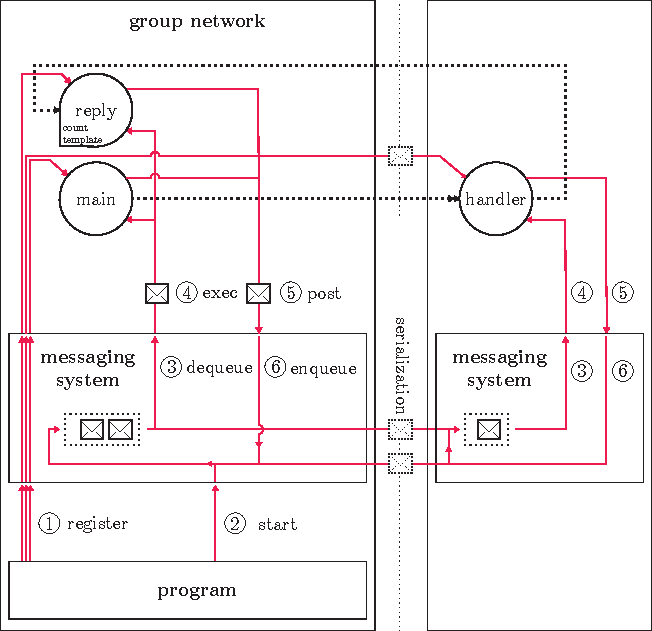
\includegraphics[width=0.7\linewidth]{../resources/schema-message.pdf}%
    \caption{The fluxional execution model in details}%
    \label{fig:MesSys}%
  }%
\end{figure}

The chain of functions from listing \ref{lst:source} is expressed in the fluxional language in listing \ref{lst:fluxional}.
The fluxion \texttt{handler} doesn't have any dependencies, so it can be executed in a parallel event-loop.
The fluxions \texttt{main} and \texttt{reply} belong to the group \texttt{grp\_res}, indicating their dependency over the variable \texttt{res}.
The group name is chosen arbitrarily.
All the fluxions inside a group are executed sequentially on the same event-loop, to protect the shared variables against concurrent accesses.

The variable \texttt{res} is created and consumed within a chain of \textit{post} stream.
Therefore, it is exclusive to one request and cannot be propagated to another request.
It doesn't prevent the whole group from being replicated.
However, the fluxion \texttt{reply} depends on the variable \texttt{count} created upstream the \textit{start} stream, which prevents this replication.
If it did not rely on this variable, the group \texttt{grp\_res} would be stateless, and could be replicated to cope with the incoming traffic.

\separator

This execution model allows to parallelize the execution of an application as a pipeline, as with the fluxion \texttt{handler}.
And some parts are replicated, as could be the group \texttt{grp\_res}.
This parallelization improves the efficiency of the application.
Indeed, as a fluxion contains its state and expresses its dependencies, it can be migrated.
It allows to adapt the number of fluxions per core to adjust the resource usage in function of the desired throughput.

Yet, the parallelization is limited by the dependencies between fluxions.
A developer can ignore these dependencies at first, to focus on productivity.
And then continuously tune the implementation to remove these dependencies and improve efficiency.
This continuous tuning avoids the disruptive shifts of technology required by current platforms.
